% datastruct/skiplist.tex
% mainfile: ../perfbook.tex
% SPDX-License-Identifier: CC-BY-SA-3.0

\QuickQuizChapter{chp:Data Structures: Skip lists}{Data Structures: Skip Lists}{qqzdatastructskiplist}
%
\Epigraph{I think that I shall never see \\
	  A poem lovely as a tree.}
	 {Joyce Kilmer}

The preceding chapter focused on data structures that enhance
concurrency due to partitionability
(\cref{sec:datastruct:Partitionable Data Structures}
on
\cpageref{sec:datastruct:Partitionable Data Structures}),
efficient handling of read-mostly access patterns
(\cref{sec:datastruct:Read-Mostly Data Structures}
on
\cpageref{sec:datastruct:Read-Mostly Data Structures}),
or application of read-mostly techniques to avoid
non-partitionability
(\cref{sec:datastruct:Non-Partitionable Data Structures}
on
\cpageref{sec:datastruct:Non-Partitionable Data Structures}).
One of the hash table's greatest advantages for parallel use is that it
is fully partitionable, at least while not being resized.
However, it does not preserve locality of reference (unless said
locality is hash-function-aware) and it does not support key-order
traversals.

One way of gaining locality of reference and key-order traversal
to use a tree.
But use of trees in concurrent software raises some questions:

\begin{enumerate}
\item	Can trees support concurrent updates, which is trivially
	provided by hash tables?
\item	Trees avoid hash-table resizes, but often require
	rebalancing.
	Can this rebalancing be avoided?
\item	If rebalancing is necessary, can it be carried out while
	preserving performance and scalability for both readers
	and updaters?
\end{enumerate}

One such tree is the radix tree, which is also called a trie.
Tries partition the search key, using each successive key partition
to traverse the next level of the trie.
As such, a trie can be thought of as a set of nested hash tables,
thus providing the required concurrent updates.
Although tries do not require rebalancing, a sparse key space can result
in inefficient use of memory.
There are a number of compression techniques that may be used to
work around this disadvantage, including hashing the key value to
a smaller keyspace before the
traversal~\cite{RobertOlsson2007Trash}.
Radix trees are heavily used in practice, including in the Linux
kernel~\cite{NickPiggin2006radixtree}.
However, because of their similarity to hash tables, this chapter
will not say more about them.

One important special case of both a hash table and a trie is what is
perhaps the oldest of data structures, the array and its multi-dimensional
counterpart, the matrix.
The fully partitionable nature of matrices is exploited heavily in
concurrent numerical algorithms, as we saw in
\cref{sec:SMPdesign:Locking Granularity and Performance}
on
\cpageref{sec:SMPdesign:Locking Granularity and Performance}.
This chapter will nevertheless focus on linked data structures.

Self-balancing trees are heavily used in sequential code, with
AVL trees and red-black trees being perhaps the most well-known
examples~\cite{ThomasHCorman2001Algorithms}.
Early attempts to parallelize AVL trees were complex and not necessarily
all that efficient~\cite{Ellis80},
however, more recent work on red-black trees provides better
performance and scalability by using RCU for readers and hashed arrays
of locks\footnote{
	In the guise of swissTM~\cite{AleksandarDragovejic2011STMnotToy},
	which is a variant of software transactional memory in which
	the developer flags non-shared accesses.}
to protect reads and updates,
respectively~\cite{PhilHoward2011RCUTMRBTree,PhilipWHoward2013RCUrbtree}.
It turns out that red-black trees rebalance aggressively, which works
well for sequential programs, but not necessarily so well for parallel
use involving frequent updates.
Recent work has therefore made use of RCU-protected ``bonsai trees''
that rebalance less aggressively~\cite{AustinClements2012RCULinux:mmapsem},
trading off optimal tree depth to gain more efficient concurrent updates.
However, efficiently and scalably handling rebalancing is still somewhat
of a research topic, so this chapter will look elsewhere.

@@@ Btree and Maple tree.

Concurrent skip lists lend themselves well to concurrent rebalancing,
to RCU readers, and to concurrent updates.
In fact skiplists were an early academic use of a technique resembling
RCU~\cite{Pugh90}.
This chapter will therefore focus on concurrent RCU-protected skip lists.

@@@
Because this chapter cannot delve into the details of every concurrent
data structure,
\cref{sec:skiplist:Other Data Structures}
surveys a few of the important ones.
@@@

\begin{figure}
\centering
\resizebox{3in}{!}{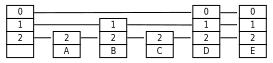
\includegraphics{datastruct/skiplistlayout}}
\caption{Skiplist Diagram}
\label{fig:datastruct:Skiplist Diagram}
\end{figure}

\section{Other Data Structures}
\label{sec:skiplist:Other Data Structures}
%
\epigraph{All life is an experiment.
	  The more experiments you make the better.}
	 {Ralph Waldo Emerson}

Concurrent double-ended queues were discussed in
\cref{sec:SMPdesign:Double-Ended Queue},
and concurrent stacks and queues have a long history~\cite{Treiber86},
though not normally the most impressive performance or scalability.
They are nevertheless a common feature of concurrent
libraries~\cite{PaulMcKenney2013LWNURCUqueuestack}.
Researchers have recently proposed relaxing the ordering constraints
of stacks and queues~\cite{Shavit:2011:DSM:1897852.1897873},
with some work indicating that relaxed-ordered queues actually have
better ordering properties than do strict FIFO
queues~\cite{AndreasHaas2012FIFOisnt,ChristophMKirsch2012FIFOisntTR,AndreasHaas2013CFRelaxedQueues}.

It seems likely that continued work with concurrent data structures will
produce novel algorithms with surprising properties.

That said, performance and scalability are of little use without reliability,
so the next chapter covers validation.

\QuickQuizAnswersChp{qqzdatastructskiplist}
